% Copyright (c) 2014,2016,2018 Casper Ti. Vector
% Public domain.

\chapter{\emph{decryst}:高效的粉晶结构测定软件}\label{chap:decr-theory}
\section{\emph{decryst} 中的增量计算}\label{sec:decr-incr}

如第 \ref{sec:atom-bump} 节所述,针对成键关系总体未知的结构,为了提升排除原子
重叠的效率,本人基于第 \ref{chap:cryst-cd} 章中的机制开发了 \emph{decryst}。
本人在开发 \emph{decryst} 的过程中,通过应用增量计算的思想,使其全局最优化
步骤的性能得到了大幅度的提升(参考第 \ref{ssec:incr-obj} 小节);除此之外,
通过增量生成等效点系组合,本人极大地降低了 \emph{decryst} 的内存需求(参考第
\ref{ssec:incr-epc} 小节)。此外,在讨论这些问题之前,第 \ref{ssec:incr-intro}
小节将简要回顾 \emph{decryst} 中应用的和增量计算相关的技术。

\subsection{增量计算和惰性计算}\label{ssec:incr-intro}

\myterm{增量计算}的思想在计算机科学技术的发展中有着深远的影响:于 70 年代
后期出现在 Unix 中的 \verb|make| 程序\parencite{feldman1979}会检测软件
项目中发生变更的模块,然后执行命令根据依赖关系重新构建所有受影响的模块(图
\ref{fig:make-build}),从而避免重复构建未发生变更的模块;于 2016 年推出的视频
游戏 \emph{Doom} 中,通过在渲染每一帧画面时巧妙地利用为前一帧画面计算的数据,制
作方将游戏的画面品质和图形性能提升到了新的水平\parencite{correges2016}。有必要
指出,增量计算和\myterm{惰性计算}是一脉相承的,因为合理地避免多余的计算可以说
正是惰性计算的核心思想;受此启发,在 \emph{decryst} 中,除了增量计算之外,本人
也应用了其它的可归类为惰性计算的技术,而本小节将对这些技术进行简短的总结。

\begin{figure}[htbp!]\bfcmd
\ffigbox{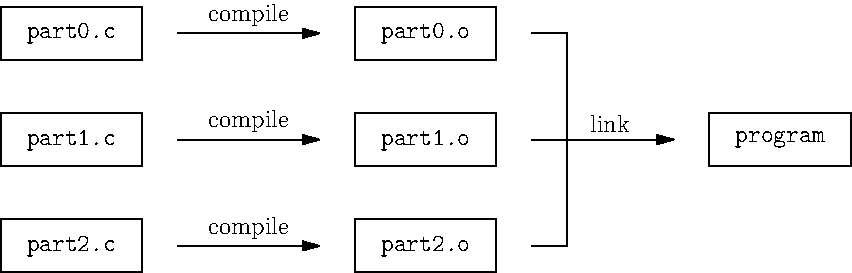
\includegraphics[width = 0.64\textwidth]{img/make-build}}{\caption[%
	\texttt{make} 如何构建一个示例程序%
]{%
	\texttt{make} 如何构建一个示例程序:在 \texttt{program} 构建完成之后,
	如果 \texttt{part0.c} 发生变更,为了再次构建 \texttt{program},\texttt{make}
	只须重新编译 \texttt{part0.c} 然后重新链接所有 \texttt{.o} 文件%
}\label{fig:make-build}}
\end{figure}

首先,本人认为代码中处理对象的分离(separation of concerns)和惰性计算的思想是
符合的:例如全局最优化的代码不应该关心结构中所涉及化学元素的名称和符号,更不应该
关心在绘制结构图时使用什么颜色的球体来表示其中的原子。通过对各模块所处理对象的
细致分离,我们不仅会使软件的架构更加清晰,也会减少各模块代码所从事的无用工作,
因此在增强软件可维护性的同时也提升了软件的性能。在 \emph{decryst} 的架构设计中,
这一原则的一些具体体现可以参考第 \ref{ssec:decr-arch} 小节。

其次,CPU 缓存\parencite{bryant2011}可以认为是一种通过硬件实现的惰性计算技术,
这一技术使得对连续内存区域的访问被定向到访问效率远快于内存的缓存,从而提升程序
性能。相应地,利用 CPU 缓存的方法是使用对缓存友好的算法和数据结构,从而尽量
利用连续的内存区域:例如在可行的前提下,尽量使用快速排序算法而非归并排序算法
(参考第 \ref{ssec:cryst-sap} 小节),使用数组而非链表,等等。

根据增量计算避免重新计算未改变值的思想,对于值不发生改变的函数,在首次求值
之后便不须重新求值了;而如果将这些函数的求值提前到程序的开头,我们所做的
就是建立查找表。对于计算开销很大的函数,使用查找表显然十分有利:
例如在正空间法的全局最优化步骤中,对于 X 射线原子散射因子
\begin{equation}
	f_\mathrm{X}(hkl) = g_\mathrm{X}(\sin\theta_{hkl} / \lambda)
	= c_\mathrm{X} + \sum_i a_{\mathrm{X},i} \iee ^
		{b_{\mathrm{X},i} (\sin\theta_{hkl} / \lambda) ^ 2}\mccomma
\end{equation}
注意到其求值须要多次用到计算较慢的指数函数和正弦函数,其计算开销显然很大;
又因为其值只取决于衍射指标 $hkl$、元素 X 和在最优化步骤中不变的波长
$\lambda$,所以其特别适合使用查找表。因为上述原因,\emph{decryst}
会在最优化程序的一开始建立包括原子散射因子在内若干函数的查找表。

\emph{decryst} 使用模拟退火作为其全局最优化算法,而后者可以和物理退火相类比:
既然保温可以让系统趋于平衡,如果在系统始终不太远离平衡的前提下逐渐降低温度,就
可以期望使系统接近低温下的平衡态。显然,如果系统已经很接近平衡,就不必再保温,
这样可以减少非必要的保温过程所花费的时间,而这正是自适应模拟退火的思路:不是在
每个温度阶梯上保温固定的时间,而是在检测到系统接近平衡时自动降温。就目前而言,%
\emph{decryst} 在其最优化步骤中使用的是 \textcite{lam1988}的自适应模拟退火
算法,因为对后者可以比较方便地进行并行化(参考第 \ref{ssec:decr-para} 小节)。

最后,注意到晶胞中常有的对称性,以及结构因子的计算开销在全局最优化总开销
中的高权重(参考第 \ref{ssec:incr-obj} 小节),\emph{decryst} 中也利用
以下关系来降低结构因子的计算开销(其中 $\vec{q}$ 为散射向量):
\begin{equation}
	F_\text{反演对称}(\vec{q}) = \sum_i f_i(\vec{q}) (
		\iee ^ {2\uppi\eye\vec{q} \cdot \vec{x}_i} +
		\iee ^ {2\uppi\eye\vec{q} \cdot (-\vec{x}_i)}
	) = 2\sum_i f_i(\vec{q}) \cos(2\uppi\vec{q} \cdot \vec{x}_i)
	\mccomma\label{eq:cent-sym}
\end{equation}
其中 $i$ 为中心对称原子对的编号;
\begin{equation}
	F_\text{带心格子}(\vec{q}) = \sum_{ij} f_i(\vec{q})
		\iee ^ {2\uppi\eye\vec{q} \cdot (\vec{x}_i + \vec{r}_j)}
	= \sum_i f_i(\vec{q}) \iee ^ {2\uppi\eye\vec{q} \cdot \vec{x}_i}
		\sum_j \iee ^ {2\uppi\eye\vec{q} \cdot \vec{r}_j}\mccomma
\end{equation}
其中 $\vec{r}_j$ 为可选原点的坐标。

最后有必要指出,惰性计算技术或多或少地在其它晶体学软件中有所应用,而且其对软件
性能的影响是较为显而易见的,但本人未能找到一个较为全面的对以上技术的总结。这样的
现状所造成的一个不良的结果是部分晶体学软件对这些技术的忽视,例如 \emph{EPCryst}%
\parencite{deng2011}在上述技术中只应用了查找表这一项技术,这使得其在 \ce{PbSO4}
正确等效点系组合的全局最优化中比 \emph{decryst} 慢了两个数量级\footnote{%
	根据本人的测试,在 Intel i7-3720QM CPU 上,\emph{EPCryst}
	耗时多于 \SI{1000}{\second},而 \emph{decryst}
	即使在不用增量计算的前提下耗时也少于 \SI{10}{\second}。%
}。
正因如此,本人希望本小节中的总结能对晶体学软件的设计者有所帮助。

\subsection{目标函数的增量计算}\label{ssec:incr-obj}

因为 \emph{decryst} 使用 (\ref{eq:obj-func}) 式中的函数 $E$ 作为全局最优化的目标
函数(参考第 \ref{ssec:eval-func} 小节),为了加速最优化,我们事实上须要加速
Bragg $R$ 因子和原子重叠评估函数 $B$ 的计算;又因为计算 $R$ 因子时大部分时间
用在计算结构因子上,我们显然须要加速结构因子的计算。考虑到两个相邻的最优化循环中
晶体模型之间的差别只在于某一个独立原子位置的移动,根据 Fourier 变换的可加性有
\begin{equation}
	F'(\vec{q}) - F(\vec{q}) = \sum_i f_i(\vec{q}) (
		\iee ^ {2\uppi\eye\vec{q} \cdot \vec{x}'_i}
		- \iee ^ {2\uppi\eye\vec{q} \cdot \vec{x}_i}
	)\mccomma
\end{equation}
其中 $i$ 是被移动原子的编号。根据这一关系,我们可以利用前一晶体模型的结构因子
数据增量地计算后一晶体模型的结构因子:只须对被移动的原子重新计算 $\iee ^
{2\uppi\eye\vec{q} \cdot \vec{x}_i}$ 项的值即可。由此可知,如果晶胞中有 $m$
个独立原子,而这些原子在各最优化循环中被轮流移动,那么晶胞中所有原子结构因子的
重新计算将被 $m$ 个最优化循环分担(而非原先的在单个最优化循环中完成),于是结构
因子的计算性能将是原先算法的 $m$ 倍。

类似地,对于 $B$ 所依赖的两体势 $C$(参考 \ref{eq:two-body} 式),显然其中对势
函数 $c(k_0, k_1)$ 的值只在 $\{k_0, k_1\}$ 对中至少一个原子被移动时发生改变;
因此 $C$ 的值也可以增量地计算,只须对上述原子对重新进行碰撞检测和处理即可。又注
意到利用等效点系对称性(参考第 \ref{ssec:ep-sym} 小节),我们只须对含独立原子的
原子对进行碰撞检测,所以最终细碰撞检测次数的上限是 $(n - 1) + (m - 1)(n' - 1)$,
其中 $n$、$m$、$n'$ 分别为晶胞的总内原子数、独立原子数和被移动独立原子的等效
原子数。在平均意义下,上述碰撞检测的时间复杂度是 $O(n)$ 量级,因此我们不再须要
专门使用类似于 sweep and prune(参考第 \ref{ssec:cryst-sap} 小节)的粗碰撞检测
算法以避免逐对碰撞检测的 $O(n^2)$ 复杂度,这在上述 SAP 算法常数因子较大的背景
之下尤其值得注意;相应地,因为不再须要计算原子的投影区间,我们也就不再须要使用
原子缩放因子,而是只需要对缩放因子。此外有必要特别提请注意的是,当最优化
循环的次数很大时,增量求和的浮点数误差积累可能会造成严重的问题,而类似于
\textcite{kahan1965}算法的增量浮点数求和算法难以应用,因为被求和数的
平均值渐进地趋于零\parencite{higham1993}。就目前而言,\emph{decryst}
通过在增量求和中使用定点数来绕过这一问题,因为定点数算术是没有误差的。

最后,本人在 Intel i7-3720QM CPU 上就增量计算对全局最优化步骤性能的影响
进行了测评。除了可以从项目主页 \url{https://gitea.com/CasperVector/decryst}
获取的数据之外,其它测试数据可以从文献\parencite{liu2018}的补充材料中获取。
本人从 AMCSD 数据库\parencite{downs2003}中获取了若干个不同复杂度的结构,
并对这些结构计算了目标函数:具体而言,对于每一个测试结构,本人测试了 100 组
晶体模型,每组由 100 个通过为独立原子赋予随机坐标的方式生成的模型构成。
本人度量了在使用或不使用增量计算(分别对应于 $t_{\cdots,\text{incr}}$ 和
$t_{\cdots,\text{orig}}$)时对每组模型计算整个目标函数 $E$ 或只是 Bragg $R$
因子所花费时间(分别对应于 $t_{E,\cdots}$ 和 $t_{R,\cdots}$)的平均值和
标准差,并将其除以每组的模型数,结果如表 \ref{tbl:incr-eval} 所述。

\begin{table}[htbp]\bfcmd
\sisetup{table-number-alignment = center}
\ttabbox{\begin{tabular}{
	crrr@{\extracolsep{1.5em}}
	S[table-format = 2.4]@{\extracolsep{1em}}
	S[table-number-alignment = center-decimal-marker]@{\extracolsep{1.25em}}
	S[table-format = 2.4]@{\extracolsep{1.25em}}
	S[table-number-alignment = center-decimal-marker]
}\toprule
ID &	$n$ &	$m$ &	$N_\text{refl}$ &	{$t_{R,\text{incr}}$} &
{$t_{R,\text{orig}}$} &	{$t_{E,\text{incr}}$} &	{$t_{E,\text{orig}}$} \\\midrule
0005558 &	24& 5& 94 &	8.9(3) &	43.9(5) &	12.5(7) &	44.5(7) \\
0009272 &	64& 8& 80 &	39.7(9) &	241(3) &	50.6(6) &	242(3) \\
0009563 &	90& 10& 76 &	15.0(2) &	168(3) &	30.0(7) &	174(2) \\
0002630 &	126& 14& 73 &	11.3(3) &	244(3) &	30.7(3) &	252(2) \\
0000427 &	152& 20& 374 &	27.4(5) &	639(7) &	53.6(7) &	663(8) \\
0000447 &	160& 4& 32 &	27.0(9) &	87(2) &	59(1) &	102(2) \\\bottomrule
\end{tabular}}{\caption[\emph{decryst} 中增量计算的性能测评]{%
	\emph{decryst} 中增量计算的性能测评(时间单位为 \si{\micro\second}):ID
	为测试结构在 AMCSD 中的代号,$n$ 和 $m$ 分别为晶胞中的总原子数和独立原子
	数,$N_\text{refl}$ 为有记录的衍射峰数;$t_{E,\cdots}$ 和 $t_{R,\cdots}$
	分别为计算每个模型 $E$、$R$ 所需的时间; $t_{\cdots,\text{incr}}$ 和
	$t_{\cdots,\text{orig}}$ 分别为用或不用增量计算时所需的时间。%
}\label{tbl:incr-eval}}
\end{table}

从表中可见,对于各个复杂度的测试结构,$R$ 因子和 $B$ 的计算性能都因增量计算的
应用而得到了极大(有时多于一个数量级)的提升。有必要指出,表中“0009272”的测试
结果和“0000447”的 $t_{\cdots,\text{orig}}$ 可能显得反常,但事实上前者可以从
相应结构并非带心格子以及其中用到的 Wyckoff 位置均没有中心对称性(参考第
\ref{ssec:incr-intro} 小节)得到解释,而后者可以从相应结构中和 $n$ 相比
很小的 $m$(参考第 \ref{ssec:ep-sym} 小节)以及和其它结构相比
很小的 $N_\text{refl}$ 得到解释。

\subsection{等效点系组合的增量生成}\label{ssec:incr-epc}

考虑生成 \ce{Al2O3}($R\bar3c$,菱方表示下 $Z = 2$)等效点系组合(EPC)的问题:
其空间群具有 $2a$、$2b$、$4c$、$6d$、$6e$、$12f$ 等共 6 种 Wyckoff 位置,其中
$2a$、$2b$ 位置因为坐标完全固定所以不能被多次占据,否则必然发生极其严重的原子
重叠。在这样的约束下,其总共有 6 个可行 EPC:$a_1b_1/d_1$,$a_1b_1/e_1$,%
$c_1/a_1c_1$,$c_1/b_1c_1$,$c_1/d_1$ 和 $c_1/e_1$(其中 $a_1b_1/d_1$ 是
[\ce{Al^{3+}}: $2a\times1+2b\times1$; \ce{O^{2-}}: $4d\times1$] 的简写,
其余类似;$c_1/e_1$ 为正确 EPC)。对于同样空间群的 \ce{A2B3},\ce{A2B3C3},%
\ce{A2B3C3D3},$\cdots$,这一系列结构的可行 EPC 数随着元素数的增长接近于指数增
长:6,16,38,78,142,236,366,$\cdots$;对于 Wyckoff 位置种类较多的空间群,
特别是以 $Pmmm$ 为代表的一些正交晶系空间群,可行 EPC 数过大的问题尤为突出。

在 \textcite{deng2009}原先提出的 EPC 生成算法中,每个元素的可行 EPC 被单独生
成,然后这些单元素 EPC 被组合成总的 EPC,这样的做法显然须要存储各元素可行 EPC
的列表以便在生成总 EPC 时使用;此外,\emph{EPCryst}\parencite{deng2011}将
单元素可行 EPC 和总可行 EPC 的列表存储在内存中,因此其在可行 EPC 数很大时可能
遇到内存溢出的问题。为了应对这一问题,\emph{decryst} 使用了增量的方式生成可行
EPC,并直接将得到的每个总可行 EPC 输出到文件,从而避免内存溢出,
而本小节将对增量生成 EPC 的算法进行讨论。

首先考虑 \ce{Al2O3} 中 \ce{Al^{3+}} 可行 EPC 的生成:如图 \ref{fig:epc-tree}
所示,在人工搜索 \ce{Al^{3+}} 的可行 EPC 时,一般的顺序是 $a_0b_0 \rightarrow
a_1b_0 \rightarrow a_0b_1 \rightarrow a_1b_1 \rightarrow \cdots$,而这样的顺序
事实上正是对一棵以 EPC 为叶节点的树进行\myterm{深度优先搜索}(depth-first
search;参考 \cite[603-612]{cormen2009})的顺序;当搜索到恰好完全符合晶胞内
\ce{Al^{3+}} 原子数的节点时(例如图中的 $a_1b_1$),就输出该节点的 EPC。显然,
一个首先需要关心的问题是如何确定搜索的限度:例如,为什么图中在搜索到 $a_1b_0$
之后紧接着搜索到的是 $a_0b_1$,而不是 $a_2b_0$?事实上,在对树进行搜索时,
往往可以根据所关心问题的数学性质进行\myterm{剪枝}(pruning),即自动排除一些
可以严格证明不需要搜索的子树\footnote{%
	在计算机科学中,一个孤立的根节点也被认为是一棵树%
	\parencite[176]{cormen2009},因此这里的“子树”也包含单一叶节点的情形。%
}。

\begin{figure}[htbp!]
\begin{floatrow}
\setlength{\columnsep}{3em}
\ffigbox[0.37\textwidth]{\begin{forest}
	[$(c_0d_0e_0f_0)$
		[$b_0$ [$a_0b_0$] [$a_1b_0$]]
		[$b_1$ [$a_0b_1$] [$\wyck1a\wyck1b$]]
	]
\end{forest}}{\caption[EPC 的生成被建模为深度优先树搜索]{%
	\ce{Al2O3} 中 \ce{Al^{3+}} 原子 EPC 的生成被
	建模为深度优先树搜索(粗体为搜索到的可行 EPC)%
}\label{fig:epc-tree}}
\ffigbox[0.37\textwidth]{\begin{forest}
	[$(a_1b_1/)$
		[$f_0$
			[$e_0f_0$ [$\cdots$]]
			[$e_1f_0$ [$\cdots$]]
			[$e_2f_0$, prune]
		] [$f_1$, prune]
	]
\end{forest}}{\caption[EPC 树搜索中根据晶胞化学式进行的剪]{%
	EPC 树搜索中根据晶胞化学式进行的剪枝(浅色为被剪掉的子树)%
}\label{fig:epc-prune}}
\end{floatrow}
\end{figure}

首先如上文所述,为了避免原子重叠,所有的固定 Wyckoff 位置(例如 \ce{Al2O3}
所属空间群的 $2a$、$2b$ 位置)分别最多只能被占据一次,因此这类位置被占据
多于一次的子树都可以剪掉,而这就是图 \ref{fig:epc-tree} 中在 $a_1b_0$ 之后
紧接着搜索到 $a_0b_1$ 的原因。除此之外,根据晶胞化学式也可以进行剪枝:例如在
图 \ref{fig:epc-prune} 中,因为 \ce{Al2O3} 的晶胞化学式不允许 $6e$ 位置被占据
多于一次,且不允许 $12f$ 位置被占据,所以相应 EPC 为 $a_1b_1/e_nf_0$($n > 1$)
和 $a_1b_1/f_n$($n > 0$)的子树都可以剪掉;值得注意的是,在使用这一剪枝
策略之后,\emph{decryst} 使用的 EPC 生成算法不再须要像 \textcite{deng2009}%
原先的算法那样预先计算单个元素 EPC 中各 Wyckoff 位置可占据次数的上限。
在 \emph{decryst} 使用的 EPC 生成算法中,以上两个策略是进行剪枝的基础。

在实际生成单元素可行 EPC 时,因为固定 Wyckoff 位置的约束是对固定位置各自总
占据数的约束,在剪枝时必须考虑其它元素 EPC 中各固定位置被占据的次数:例如在图
\ref{fig:elem-epc} 中,尽管被生成的是 \ce{O^{2-}} 的可行 EPC,程序仍须考虑
\ce{Al^{3+}} 的 EPC;因为后者占据 $a_1b_1$,所以程序可以将所有占据了 $2a$、$2b$
的子树剪掉。注意到用户可能须要根据自己的晶体学知识对 EPC 施加额外的限制,在生成
EPC 时须要支持额外设置各 Wyckoff 位置占据数的上下限,包括对单个元素占据数的限制
和对所有元素占据数之和的限制;显然,这里设置的上限也可以通过剪枝实现,
其剪枝策略和上述策略完全类似,只是在生成单元素可行 EPC
时剪枝策略中不须要考虑其它元素单独的占据数限制。

\begin{figure}[htbp!]
\begin{floatrow}
\setlength{\columnsep}{3em}
\ffigbox[0.37\textwidth]{\begin{forest}
	[$(a_1b_1/c_0d_0e_0f_0)$
		[$b_0$ [$a_0b_0$] [$a_1b_0$, prune]]
		[$b_1$, prune]
	]
\end{forest}}{\caption[单元素 EPC 的生成]{%
	单元素 EPC 的生成(注意剪枝时须考虑其它
	元素 EPC 中各 Wyckoff 位置被占据的次数)%
}\label{fig:elem-epc}}
\ffigbox[0.37\textwidth]{\begin{forest}
	[{(若要求至少一个 $2a$\\且没有 $6d$、$6e$)},
		align = center, parent anchor = south
		[$a_1b_1/$]
		[$c_1/$ [$\wyck1c/\wyck1a\wyck1c$] [$c_1/b_1c_1$]]
	]
\end{forest}}{\caption[总 EPC 的生成]{%
	总 EPC 的生成(注意其中以可行的单元素 EPC 作为树中的节点)
}\label{fig:full-epc}}
\end{floatrow}
\end{figure}

总 EPC 的生成也可以建模为树搜索,只是此时树中的节点须要换成单元素可行 EPC。
例如在搜索 \ce{Al2O3} 的总可行 EPC 时(图 \ref{fig:full-epc}),程序首先会搜索
\ce{Al^{3+}} 的可行 EPC,于是找到 $a_1b_1$;其接着在 \ce{Al^{3+}} 占据 $a_1b_1$
的前提下搜索 \ce{O^{2-}} 的可行 EPC,但因 $6d$、$6e$ 位置占据数上限为零的约束%
\footnote{这显然和 \ce{Al2O3} 实际的 EPC 不符;这样设定纯粹是为了方便演示。}%
而找不到,于是回溯到对 \ce{Al^{3+}} 可行 EPC 的搜索。类似于以上的步骤,程序最终
会搜索到指定约束下所有的总可行 EPC。至此,我们还没有考虑的问题只剩占据数的
下限约束,其中单元素下限约束显然可以在搜索单元素可行 EPC 时通过剪枝实现;
总占据数的下限约束因为无法在搜索单元素可行 EPC 时实现,所以只能在生成
总可行EPC 时通过对结果的额外筛选实现,例如图中 $c_1/b_1c_1$ 就是因为
$2a$ 位置至少占据一次的约束而被筛除的。

有必要指出,由本小节可见,增量计算不仅可以用于降低算法的时间复杂度,而且在特定的
条件下也可以用于降低算法的空间复杂度。此外,\emph{decryst} 使用的 EPC 生成算法
在性能上未必优于 \emph{EPCryst} 中的算法,但正空间法的性能瓶颈并不在 EPC 的
生成上,因此用其性能上的降低来换取整套软件在内存需求上的极大缩减还是很有利的。
最后,本人将本小节的算法归类为增量算法,其理由有两条:第一,这一算法不再使用一个
分离的步骤专门生成单元素可行 EPC,而是利用树搜索模型动态地生成总可行 EPC;第二,
在这一算法的具体实现中,\emph{decryst} 使用的是迭代式而非递归式的树搜索,
因此程序会从前一 EPC 计算后一 EPC,而这正是增量式的计算。

\section{\emph{decryst} 设计简介}
\subsection{\emph{decryst} 中的并行化}\label{ssec:decr-para}

增量计算的基础是数据之间依赖关系的相对独立性,例如图 \ref{fig:make-build} 中
\verb|part0.c| 变更后其余 \verb|.c| 文件不需重新编译的根本原因在于数据的变更只
影响反向依赖(以及反向依赖的反向依赖,等等)。实际工作中遇到的依赖关系往往更加
复杂多变,例如像图 \ref{fig:topo-sort} 中所示的情形;幸运的是,\emph{decryst}
中许多关键计算环节(例如第 \ref{ssec:incr-obj} 小节中分析的那些)的依赖关系
可以归纳为(图 \ref{fig:map-reduce})一组互相独立的计算结果(图中的 $f(x_i)$)
被集中汇总(图中的“$\oplus$”操作)。事实上,这种相对独立性在很大程度上也是
并行化的基础:例如要是在 \verb|make| 程序构建软件项目时启用了并行选项,
那么 \verb|make| 会根据依赖关系并行地执行互相独立的计算步骤。对于图
\ref{fig:map-reduce} 中的依赖模式,其中被汇总的各项数据在一定前提下
是互相独立的,因此可以并行地计算;这正是目前在并行和分布式计算中
被广泛应用的 MapReduce\parencite{dean2004}框架的基础,而
\emph{decryst} 中的并行化也是基于这一模式。

\begin{figure}[htbp!]\bfcmd
\begin{floatrow}
\setlength{\columnsep}{2.5em}
\ffigbox[\FBwidth]%
	{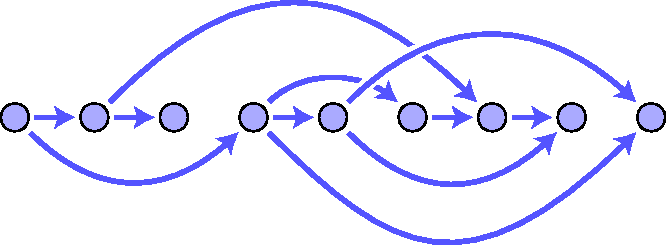
\includegraphics[width = 0.45\textwidth]{img/topo-sort}}
	{\caption{复杂依赖关系示例}\label{fig:topo-sort}}
\ffigbox[\FBwidth]%
	{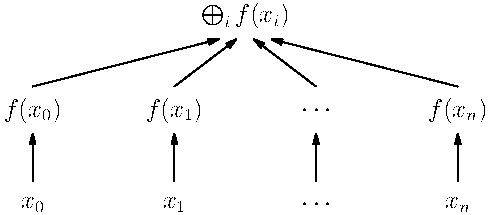
\includegraphics[width = 0.45\textwidth]{img/map-reduce}}
	{\caption{MapReduce 式依赖关系}\label{fig:map-reduce}}
\end{floatrow}
\end{figure}

类似于 \emph{EPCryst}\parencite{deng2011},\emph{decryst} 也使用等效点系组合
(EPC)法处理已指标化的数据,并把求解流程分为生成 EPC 列表、对各 EPC 进行统计
分析、对每个 EPC 进行全局最优化和导出解模型等 4 个主要步骤。因为各 EPC 上的任务
互相独立,所以 \emph{decryst} 可以并行地处理这些任务(图 \ref{fig:epc-para})。%
\textcite{deng2011}提到,\emph{EPCryst} 在 EPC 数较小(例如少于 100 个)且每个
EPC 的维数不超过 10 时特别适用;相比之下,因为 \emph{decryst} 中增量计算的应用
(参考第 \ref{sec:decr-incr} 节)以及 EPC 任务的并行化,其可以处理上千个 EPC,
每个 EPC 的维数可高达 20 以上。考虑到 EPC 法可以极大缩减搜索空间,
以及成键关系大体未知的结构 EPC 数往往很大,可以认为 EPC
任务的大规模并行化将为这类结构的求解带来前所未有的机遇。

\begin{figure}[htbp!]\bfcmd
\ffigbox%
	{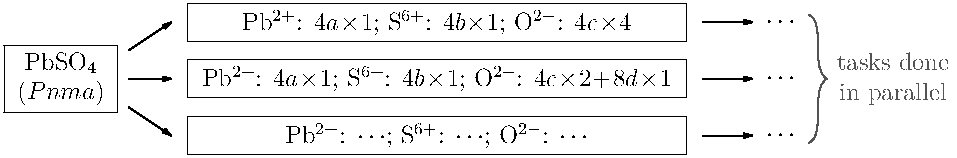
\includegraphics[width = 0.78\textwidth]{img/epc-para}}
	{\caption{EPC 的并行处理}\label{fig:epc-para}}
\end{figure}

对于维数很高的 EPC,\emph{decryst} 也可以使用并行的全局最优化,其中应用的是
\textcite{chu1999}的并行模拟退火算法,而后者又是基于 \textcite{lam1988}的
自适应模拟退火算法。Lam 算法使用连续降温,其中降温速率由若干统计参数动态控制,
而这些参数是根据相应的一套统计估计函数(statistical estimators)周期性地(每
$\tau$ 个最优化循环)计算得到的;此外为了尽量发挥最佳性能,最优化中的扰动规模
也是动态控制的,以使随机晶体模型的接受率保持在 0.44 左右。\textcite{chu1999}%
注意到模拟退火的一种物理图像是对 Boltzmann 分布的抽样,而多个抽样进程之间
可以通过周期性的状态混合来实现关联(图 \ref{fig:sa-para});
具体而言,在温度 $T$ 下选取某一进程中最近状态的概率为
\begin{equation}
	p_j = \iee ^ {-E_j / T} \Big/ \sum_j \iee ^ {-E_j / T}\mccomma
\end{equation}
其中 $E_j$ 为进程 $j$ 中最近的目标函数值。利用对各进程最近状态的周期性混合,
Boltzmann 抽样的操作可以被分配到多个进程上进行,由此便可实现对模拟退火的并行化。

\begin{figure}[htbp!]\bfcmd
\ffigbox%
	{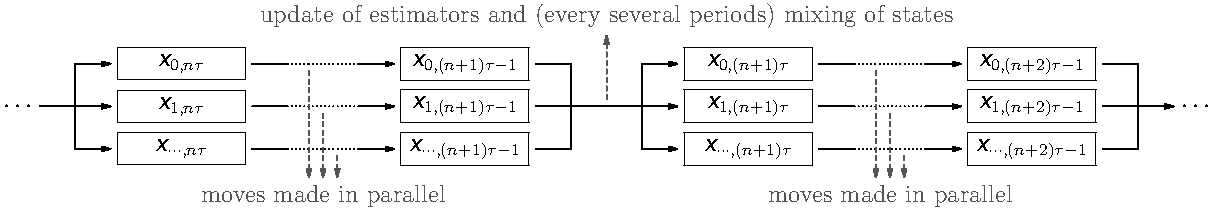
\includegraphics[width = 0.99\textwidth]{img/sa-para}}
	{\caption{模拟退火的并行化}\label{fig:sa-para}}
\vspace{\slop{-0.2em}}
\end{figure}

考虑到 \emph{decryst} 须要处理的实际需求,本人对原先并行模拟退火算法中的
一些技术细节进行了细微的改动。首先,因为晶胞具有周期边界,\emph{decryst}
中使用的搜索空间不是无限的空间,而是具有周期边界的超立方体,即多维环面(参考
第 \ref{ssec:cryst-geom} 小节);相应地,最优化中的移动步长不是从带有随机
符号的指数分布生成,而是从带有随机符号的周期指数分布(wrapped exponential
distribution)生成。其次,因为 \emph{decryst} 会随机地初始化独立原子的坐标,
所以原先算法中用于消除初态痕迹的在无限温度下进行的多次初始循环不再需要;
此外因为 \emph{decryst} 中有专门的统计分析步骤,所以用于计算统计估计函数值的
多次初始循环也不再需要。最后,为了修复或改善 \emph{decryst} 在实际测试中的
一些问题,本人还对原先算法本身进行了几项调整:

\begin{itemize}
\item 本人发现在最优化的初期,原先的算法有一定概率遇到降温过快的问题;为了解决
	这一问题,\emph{decryst} 硬性设定了模拟退火时两个相邻最优化循环中温度之比的
	上限,从而避免降温过快。本人也注意到,在最优化问题的维数很大时,特定统计参数
	的估计函数值可能被计算为浮点数中的 Inf(infinity)或 NaN(not a number),
	导致算法异常终止;为了解决这一问题,相应估计函数被适当修改\footnote{%
		具体而言,是文献\parencite[10]{lam1988}中的 $A$、$D$;同一页中的
		$\hat\mu$ 从代数上看也可能出现类似问题,因此也有类似的修改。%
	},以尽量消除计算得到的 Inf 和 NaN。此外有必要指出,上述避免降温过快的
	机制在其中也有所帮助,因为降温过快是出现 Inf 和 NaN 的一种触发条件。
\item 为了避免扰动规模 $\theta$ 在接近零时变化过于剧烈,\emph{decryst}
	中使用了基于倍数的动态控制(其中 $\rho_0$ 为最近 $\tau$
	个最优化循环所产生随机晶体模型的接受率)
	\begin{equation}
		\theta_i = \theta_{i-\tau} (\rho_0 - 0.44 + 1)\mccomma
	\end{equation}
	而不是原先基于加和的动态控制
	\begin{equation}
		\theta_i = \theta_{i-\tau} + (\rho_0 - 0.44)\mcstop
	\end{equation}
\item 在并行化中,每个进程的降温速率须为串行降温速率乘以并行进程数:例如假设串行
	温度序列为 $T_0$、$T_1$、$T_2$、$\cdots$,则原算法中双进程时每个进程的温度
	序列将为 $T_0$、$T_2$、$T_4$、$\cdots$。然而注意到一些温度值会在降温中被
	跳过,例如上述例子中的 $T_1$、$T_3$、$T_5$、$\cdots$,而这样可能造成统计估计
	函数值和实际值偏差过大,本人因此改为将串行温度序列分配到各进程,例如双进程时
	两个进程的温度序列将分别为 $T_0$、$T_2$、$T_4$、$\cdots$ 和
	$T_1$、$T_3$、$T_5$、$\cdots$。
\item 假设最优化问题的维数为 $n$,则每个最优化进程在进行 $n$ 个最优化循环之后
	会将 $n$ 个自变量的更新顺序打乱,从而消除各自变量上扰动之间的关联。这样的
	顺便带来的一个效果是每个进程中更新统计估计函数值的周期
	(即 $\tau$ 除以进程数得到的值)不再必须是 $n$ 的倍数。
\item 原先的并行化实现混合地使用了服务器{--}客户端模式和点对点模式来实现
	计算节点之间的通信。考虑到点对点模式在这一算法中对性能影响并不大,
	本人在 \emph{decryst} 的全局最优化步骤中统一采用了服务器{--}客户端模式,
	以本机为进行汇总操作的客户端、计算节点为进行独立计算的服务器端,
	利用 ZeroMQ 库进行通信(参考第 \ref{ssec:decr-arch} 小节)。
	事实上,这样也更接近于 MapReduce 的做法。
\end{itemize}

\subsection{\emph{decryst} 的软件架构}\label{ssec:decr-arch}

\emph{decryst} 是自由、开源的软件,可以从
\url{https://gitea.com/CasperVector/decryst} 获得。考虑到本人能力和精力有限,
难以承担“重复发明轮子”的成本,本人在开发 \emph{decryst} 时尽量将其设计得简洁、
灵活,从而可以关注其核心功能的开发。本人衷心希望其中应用的各种技术能够被晶体学
同行研究学习,并最终在更多的晶体学软件中得到实际的应用,由此促进晶体学软件
在自动化水平和性能上的整体进步。\emph{decryst} 由若干个部分组成(图
\ref{fig:decr-arch}),各部分的基本分工和代码组织将在本节中进行简单的介绍,
而 \emph{decryst} 的具体使用方法将在第 \ref{chap:decr-usage} 章中进行展示。

\begin{figure}[htbp!]\bfcmd
\ffigbox%
	{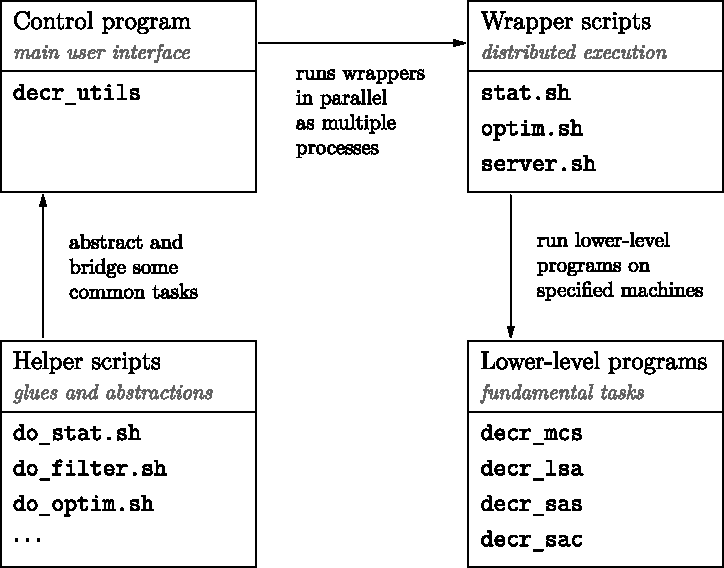
\includegraphics[width = 0.64\textwidth]{img/decr-arch}}
	{\caption{\emph{decryst} 的软件架构}\label{fig:decr-arch}}
\end{figure}

\emph{decryst} 中最基础的是一套\myterm{底层程序}(lower-level programs),其中
每一个程序实现一项底层功能:统计分析,全局最优化,等等。为了尽量发挥最佳性能,
底层程序以 C 语言写成,其代码位于 \emph{decryst} 目录树中的 \verb|src| 目录:
\begin{itemize}
\item \verb|decr_mcs|(\textbf{M}onte \textbf{C}arlo \textbf{s}tatistical
	analysis):\\实现了对单个等效点系组合(EPC)的统计分析。
\item \verb|decr_lsa|(\textbf{l}ocal \textbf{s}imulated
	\textbf{a}nnealing):\\实现了对单个 EPC 的串行模拟退火。
\item \verb|decr_sas|(\textbf{s}imulated \textbf{a}nnealing
	\textbf{s}erver):\\实现了单 EPC 并行模拟退火的服务器端。
\item \verb|decr_sac|(\textbf{s}imulated \textbf{a}nnealing
	\textbf{c}lient):\\实现了单 EPC 并行模拟退火的客户端。
\end{itemize}

建立在底层程序之上的是一个上层的\myterm{主控程序}(control program),其和
底层程序一起构成了 \emph{decryst} 的核心。主控程序调用各底层程序并和它们协作,
此外一些较为复杂但对软件总体性能影响不大的功能(特别是 EPC 的生成)
也是在主控程序中实现的。为了最大化其灵活性,主控程序以 Python 语言
写成,其代码位于 \emph{decryst} 目录树中的 \verb|python| 目录:
\begin{itemize}
\item \verb|decr_utils|:即主控程序本身;为了方便安装,本人有意将
	程序代码集中在同一文件里,但对其各部分代码进行了较为清晰的组织。
\item \verb|wyck.json|:各空间群及其中各 Wyckoff 位置的相关数据。
\item \verb|asf.json|:各元素的原子散射因子数据
	(参考第 \ref{ssec:incr-intro} 小节)。
\item \verb|rad.json|:各元素的“原子”半径(含离子半径)数据。
\end{itemize}

\myterm{包装脚本}(wrapper scripts)%
根据给定的控制参数在指定的计算节点\footnote{%
	因为 \emph{decryst} 中客户端在统计分析和全局最优化时的计算负担
	一般并不太大,所以一台机器可以同时充当客户机和计算节点。%
}上执行相应的底层程序。主控程序在调用底层程序时,事实上是通过并行地调用包装
脚本,从而使得相应的底层程序在指定的节点上执行,由此实现并行和分布式计算。
包装脚本是普通的 Unix shell 脚本,其代码位于 \emph{decryst}
目录树中的 \verb|doc/scripts| 目录:
\begin{itemize}
\item \verb|stat.sh|:用于在节点上执行 \verb|decr_mcs|。
\item \verb|optim.sh|:用于在节点上执行 \verb|decr_lsa|。
\item \verb|server.sh|:用于在节点上执行 \verb|decr_sas|。
\item \verb|ssh.sh|:以上脚本均调用该脚本以实现对远程机器的访问,
	其具体实现会调用 Unix 中的 \verb|ssh|(secure shell)程序。
\end{itemize}

\myterm{助手脚本}(helper scripts)连接不同的计算步骤,并提供上层的抽象:例如
\verb|do_rank.sh| 会根据统计分析或全局最优化的结果,利用 \textcite{deng2011}提
出的\myterm{品质因数}(figure of merit,简称 FOM)对 EPC 进行排序,从而为各 EPC
的筛选以及在后续处理中排名的确定提供依据。和包装脚本类似,助手脚本也是 shell
脚本,而其代码也位于 \emph{decryst} 目录树中的 \verb|doc/scripts| 目录;因为
助手脚本的功能较为多样,且部分脚本之间还有互相调用的关系,所以此处不再列出其
完整列表。本人有意将包装脚本和助手脚本放在 \verb|doc| 目录下,原因是它们是
\emph{decryst}灵活性的一个主要来源:在 \emph{decryst} 目前总共约 5000 行
(不计数据文件)的代码中,包装脚本和助手脚本只用了约 100 行来实现,
但在求解实际结构时用户直接调用的主要是助手脚本,而包装脚本又是
\emph{decryst} 实现分布式计算的真正基础\footnote{%
	如下文所述,ZeroMQ 只在并行模拟退火中使用,而且事实上并行模拟退火中
	也使用了 \texttt{server.sh} 来实现对服务器端的远程控制。%
}。虽然这两类脚本已经可以直接应用于实际的结构求解,但是本人希望用户能自己
读懂其中的代码,从而可以在现有脚本的基础之上进一步定制 \emph{decryst},
使之在结构测定的自动化中最大限度地发挥作用。

\emph{decryst} 的软件文档位于其目录树中的 \verb|doc| 目录:
\begin{itemize}
\item \verb|scripts| 子目录下是示例脚本,即上述的包装脚本和助手脚本。
\item \verb|usage| 子目录下是软件的用法说明,
	用户应首先阅读其中的 \verb|guide.txt|。
\item \verb|examples| 子目录下是软件用法说明中涉及的示例数据。
\end{itemize}

\emph{decryst} 还包含了几个\myterm{测评程序}(benchmark programs),包括第
\ref{ssec:cd-eval} 和 \ref{ssec:incr-obj} 小节中测评部分所涉及的一些程序,
以及一些对软件正确性的内部测试。因为须要对代码的内部结构和微观性能
进行较为准确的测试,测评程序以 C 语言写成,其代码位于
\emph{decryst} 目录树中的 \verb|bench| 目录:
\begin{itemize}
\item \verb|bench_bump| 实现了第 \ref{ssec:cd-eval} 小节中的性能测试。
\item \verb|bench_cryst| 实现了第 \ref{ssec:incr-obj} 小节中的性能测试。
\item \verb|bench_metric| 主要是对第 \ref{ssec:narrow-discus}
	小节中若干猜想的尝试性验证。
\item \verb|bench_rbtree| 是对 \emph{decryst} 在碰撞检测中所用红黑树
	(red-black tree;参考 \cite[308-338]{cormen2009})实现正确性的测试,
	因为红黑树是一个在实现时容易出细节错误的数据结构。
\end{itemize}

\emph{decryst} 为类 Unix 系统设计,而且一般不需要太多改动
就能在类似于 Cygwin 的模拟环境中运行\footnote{%
	如上文所述,虽然 \emph{decryst} 的核心部分应该不难移植到 Windows 平台,
	但是其中的包装脚本和助手脚本是普通的 Unix shell 脚本,因此也须要调用
	传统的 Unix 工具;这些工具在 Windows 下通常是由 Cygwin 等模拟环境提供,
	因此 \emph{decryst} 在 Windows 下一般需要这些模拟环境。%
};除此之外,其正确编译和安装还需要一个满足 POSIX 标准的开发环境,而
\verb|decr_sas|、\verb|decr_sac| 两个底层程序还需要 ZeroMQ 库。为了能运行
本文中的示例,用户还需要 Python、\verb|ssh| 和满足 POSIX 标准的 Unix 工具;
更加详细的安装说明可以参考 \emph{decryst} 根目录下的 \verb|README| 文件。

\section{讨论和小结}
\subsection{关于 \emph{decryst} 性能的讨论}

对于具有反演对称性的晶胞,\emph{decryst} 可以利用 (\ref{eq:cent-sym}) 式加速
结构因子的计算,从而提升最优化的性能:注意到此时只须计算半数原子所对应结构
因子的实部,计算结构因子时的性能显然是不用此公式时性能的 4 倍;因此在使用
\emph{decryst} 求解结构时,如果晶胞原点可选,应尽量使原点位于一个反演中心上。
除此之外,对于菱方晶系的结构,因为使用六方坐标系时晶胞内总原子数是使用
菱方坐标系时的 3 倍,所以为了尽量减少 \emph{decryst} 在计算原子重叠
评估函数时须要进行碰撞检测的原子对数,我们应当尽量采用菱方坐标系。

在对测量得到的衍射数据进行指标化以及确定空间群时\parencite{altomare2008a},
根据系统消光的规律对不符合实际结果的空间群进行筛除是必不可少的步骤;相应地,
在此步骤之后得到的指标化数据,例如 FullProf\parencite{rodriguez2001}产生的
\verb|.hkl| 文件中,往往包含了零强度 $hkl$ 的数据。由 (\ref{eq:total-var}) 式
可知在计算 Bragg $R$ 因子时,如果应发生系统消光的一些 $hkl$ 实际测得的强度
确实为零,那么在计算中忽略这些 $hkl$ 不会对得到的 $R$ 值产生影响。因此,
在将指标化数据转换到方便 \emph{decryst} 读取的格式时,我们可以利用一些
自动化工具删除数据中符合消光规律的零强度 $hkl$,从而一定程度地提升最优化
的性能;类似地,在适当的条件下,可以酌情忽略高角度的 $hkl$。

考虑 $R\bar3c$ 空间群(菱方坐标系,忽略反演对称)的对称操作:
\begin{gather}
	(x,y,z)\mccomma (z,x,y)\mccomma (y,z,x)\mccomma\nonumber\\
	(\bar{z}+\frac12,\bar{y}+\frac12,\bar{x}+\frac12)\mccomma
	(\bar{y}+\frac12,\bar{x}+\frac12,\bar{z}+\frac12)\mccomma
	(\bar{x}+\frac12,\bar{z}+\frac12,\bar{y}+\frac12)\mcstop
\end{gather}
注意到上述坐标中有大量重复的表达式,例如 $x$、$y$、$z$、$\bar{x}+\frac12$、%
$\bar{y}+\frac12$、$\bar{z}+\frac12$ 分别出现了 3 次,我们似乎可以通过将
表达式分组,然后在其自变量发生改变时只求值一次,后续用到时直接使用求出的值。在
\emph{decryst} 的全局最优化步骤中,考虑到两个相邻的最优化循环里晶体模型之间的差
别一般只在于单个独立原子中一个坐标的改变,这样似乎会比较有利:除了在计算结构因子
时的便利之外,在使用 sweep and prune(SAP,参考第 \ref{ssec:cryst-sap} 小节)
时,利用上述分组,我们可以只对受坐标变动影响的那些投影区间重新进行碰撞检测。
然而,在每次计算目标函数时,原子坐标事实上是在被计算一次之后便用于计算许多
$hkl$ 的结构因子,因此原子坐标的计算开销在目标函数的计算开销中所占比例不大;
此外如 \ref{ssec:incr-obj} 小节所述,\emph{decryst} 事实上并未使用 SAP,
因此以上性能调优技术带来的性能提升非常有限,所以最终未被采用。

\subsection{关于浮点数求和的讨论}

如第 \ref{ssec:incr-obj} 小节所述,\emph{decryst} 目前在增量求和时通过在内部
使用定点数的方式来绕过浮点数求和的误差积累问题;这样做并不完美,因为定点数精度
也有限,在加法超过其上界时会溢出到下界(相应地,减法可能会溢出到上界)。为了
防止溢出,\emph{decryst} 对浮点数 $x_\text{float}$ 到定点数 $x_\text{fix}$
之间的换算常数 $c \approx x_\text{fix} / x_\text{float}$ 进行了限制,以保证
求和结果的定点数表示即使在最坏情形下也不会发生溢出。然而,因为
\begin{equation}
	c \approx M_\text{fix} \Big/ \sum_i |x_{\text{float},i}|_\text{max}
\end{equation}
(其中 $M_\text{fix}$ 为定点数所用整数类型绝对值的上界),所以 $c$ 的值在
被求和数的个数很大时会很小,从而增大换算时的截断误差;这在晶胞内总原子数
$n$ 很大时尤其值得注意,因为此时被求和数的个数是 $n (n - 1) / 2$。

另外一种可能可行的思路是直接使用增量的浮点求和,但周期性地从头求和,从而
避免求和误差的无界积累;事实上,\emph{decryst} 在并行模拟退火(参考第
\ref{ssec:decr-para} 小节)中进行状态混合时,在很大程度上已经是从头计算晶体
模型的目标函数了。然而,在各种条件下如何妥善确定从头求和的周期,
还有这一周期和 \textcite{lam1988}的算法中统计估计函数的更新周期以及
\textcite{chu1999}的算法中进行状态混合的周期之间的关系应当如何把握,
这些问题在应用上述思路之前都需要仔细考虑。

使用高精度的浮点数可以大大减轻浮点数求和中的误差积累问题,但在 \emph{decryst}
中仍无法完全根治这一问题,因为其中浮点数增量求和的误差积累是无上界的,只是在用
高精度浮点数时每次求和的相对误差被很大程度地缩小了。当然,如果将高精度浮点数和
以上周期性从头求和的思路同时使用,对误差积累进行有效控制仍是很有希望做到的;
类似地,对于上文所述晶胞内总原子数 $n$ 很大的情形,如果以高精度的整数为定点数
的基础,截断误差对最终计算结果的影响应该也是可以控制在一个满意的范围之内的。

\subsection{关于等效点系组合生成算法的讨论}\label{ssec:epc-discus}

如第 \ref{sec:dspace-epc} 节所述,在早期的正空间法工作中,晶体学家以极其
具有技巧性的方式对等效点系组合(EPC)进行筛选。例如在\textcite{lu1965}关于
\ce{V2Ga5}($P4/mbm$,$Z = 2$)的工作中,作者首先根据晶胞化学式和各 Wyckoff
位置的多重度列出了可能的多重度组合:
\begin{multicols}{2}
\begin{enumerate}[label = {\Alph*.}, leftmargin = 2\parindent]
	\item $8 + 4 + 2$;
	\item $8 + 2 + 2 + 2$;
	\item $4 + 4 + 4 + 2$;
	\item $4 + 4 + 2 + 2 + 2$;
	\item $4 + 2 + 2 + 2 + 2 + 2$;
	\item $2 + 2 + 2 + 2 + 2 + 2 + 2$。
\end{enumerate}
\end{multicols}
{\noindent}因为固定 Wyckoff 位置只有 4 个,所以组合 E、F 首先被排除;接下来,因
为 $c$ 方向空间有限,$2a$、$2b$ 互斥且 $2c$、$2d$ 互斥,所以组合 B、D 也被排除。
考虑到 $c$ 方向只能容纳一个原子,$4e$、$4f$ 不可用,在多重度为 4 的 Wyckoff 位置
中只能选择 $4g$ 或 $4h$,而这导致组合 C 在 $\{220\}$ 平面一定会发生原子重叠,
所以组合 C 也被排除。对于组合 A,在排除等价 EPC 之后,作者根据特定衍射峰的强度
对剩余的可行 EPC 进行了最终的筛选。有必要指出,在不考虑除固定位置约束之外的原子
重叠因素时,\ce{V2Ga5} 总共有 428 个可选 EPC,因此仅通过人工计算将其
EPC 筛选至只剩一个已经可谓是惊人的工作。

以上的技巧并未完全在 \emph{decryst} 中得到应用。首先,以上先生成多重度组合再
生成 EPC 的思路并未在 \emph{EPCryst}\parencite{deng2011}或 \emph{decryst}%
(参考第 \ref{ssec:incr-epc} 小节)中采用,这是因为以上思路实现起来明显更加
复杂,但在算法的时间和空间复杂度上似乎并没有很大的改善。本人认为这并不说明以上
思路已经过时,而是说明其在当前的应用场景下没有充分发挥优势;在其它一些应用
场景下,这一思路仍有可能体现其独特的价值。此外,以上筛选中用到了涉及多于一个
Wyckoff 位置的占据数约束,例如“$2a$、$2b$ 位置总共最多占据一次”,
而 \emph{decryst} 目前尚不支持这样的约束。

此外有必要指出,利用第 \ref{ssec:incr-epc} 小节中剪枝的思路,从原则上看应该是
可以在生成 EPC 时根据原子重叠等因素对其进行实时筛选的,关于这一点的详细讨论
可以参考第 \ref{ssec:prune-discus} 小节。

\subsection{其它讨论}

对于在正空间法中主要以原子坐标作为全局最优化中自变量的结构测定软件,例如
\emph{FOX}\parencite{favre2002}、\emph{FraGen}\parencite{li2012}等,利用
类似于第 \ref{ssec:incr-obj} 小节所述的方法应该不难实现目标函数的增量计算,
其中也包括比 (\ref{eq:obj-func}) 式更为复杂的一些目标函数(例如考虑了配位数、
键价、配位多面体形状等等因素的那些)。然而,增量计算对于主要面向分子晶体的
正空间法软件可能并不太适用,因为这一类软件中大量使用键长、键角等等作为
最优化的自变量,而这常常会导致单个自变量的变化影响到所有原子的坐标。

尽管多数晶体学软件并不采用等效点系组合法,可完美并行的任务仍是广泛存在的:
例如第 \ref{chap:decr-usage} 章中将介绍须要多次执行全局最优化步骤,并在其
所得解中挑选最优解的复杂结构;显然,各次最优化之间是完全独立的,因此类似于第
\ref{ssec:decr-para} 小节中那样可以完美并行。最优化算法的并行化也具有重要意义:
例如结构精修中最优化算法的并行化将可以明显缩短用户等待精修结果的时间,
而本人注意到 \textcite{eremenko2017}近期的工作已经在往这一方向努力;此外,
一些最优化算法本身就比较容易并行化,例如 \emph{FOX} 中采用的并行回火算法。

本人最近也注意到,基于 \textcite{chu1999}算法中 Boltzmann 状态混合的思路,
\textcite{lou2016}近期提出了一种新的并行模拟退火算法。新算法在实现上明显比
原算法要简单,但却有更高的并行效率;但为了提升并行效率,其不再使用自适应的
模拟退火,这使其串行性能并不优于原算法。在未来版本的 \emph{decryst} 中,
本人有可能采用上述新算法来实现并行的全局最优化;
当然,并行回火等算法也将在考虑之列。

\subsection{本章小结}

基于第 \ref{chap:cryst-cd} 章中的原子重叠排除机制,本人开发了 \emph{decryst}
这一套利用正空间法和等效点系组合(EPC)法从指标化的粉末衍射数据求解晶体结构的
软件。受 Unix 中 \verb|make| 程序的启发,本人在 \emph{decryst} 中首次将增量计算
的思想以一种具有通用性的方式应用于全局最优化步骤中,使其性能得到了明显的提升;
\emph{decryst} 也使用一种增量算法生成 EPC,这不仅极大降低了其内存需求,而且
为在生成 EPC 时对其进行实时筛选做了准备。根据 \emph{decryst} 中计算步骤的相关
属性,本人在其中加入了对并行和分布式计算的支持,使之可以通过同时利用多个处理器
实现对晶体结构测定的进一步加速;考虑到同一结构的各 EPC 互相独立,而且 EPC 数在
多数有意义的情形下都相当大,\emph{decryst} 中统计分析和全局最优化任务的并行化
将为求解成键关系总体未知的结构带来前所未有的机遇。

\begin{rquote}{0.5\textwidth}
	\begingroup\setmainfont{GFS Didot}\itshape
	Ὁ βίος βραχύς, ἡ δὲ τέχνη μακρή.\endgroup\\
	(Vita brevis, ars longa.)
\end{rquote}
\rightline{--- Greek aphorism}

% vim:ts=4:sw=4
